\documentclass{article}
\usepackage[bottom=2cm, right=1.5cm, left=1.5cm, top=2cm]{geometry}
\usepackage{amsmath}
\usepackage{amssymb}
\usepackage{amsthm}
\usepackage{enumitem}
\usepackage{exercise} % Exercises Style
\usepackage{graphicx}
\usepackage{caption}
\usepackage{environ}

% Enable Code
\usepackage{minted}
\let \extra T

\newcommand{\vect}[1]{\boldsymbol{#1}}

\newcommand{\norm}[1]{\left\lVert#1\right\rVert}
\DeclareMathOperator{\Tr}{Tr}
\DeclareMathOperator{\Cov}{Cov}
\DeclareMathOperator{\Var}{Var}
\DeclareMathOperator{\E}{E}

\usepackage{fancyhdr}
\newenvironment{solution}
{\renewcommand\qedsymbol{$\blacksquare$}
\begin{proof}[Solution]$ $}{
\end{proof}}

\title{Solutions to Assignment }
\author{Rongfei Jin}
\begin{document}

\pagestyle{fancy}
\fancyhf{}%
\fancyhead[L]{\textbf{ DS5220 \ Assignment 6}}
\fancyhead[R]{\textbf{Rongfei Jin}}
\fancyfoot[C]{\thepage}%
\maketitle
\newpage

\section{Chapter 5 - Conceptual 3}

\begin{enumerate}[label=(\alph*)]


\item
K-fold CV is implemented the following way:
\begin{enumerate}
    \item Split the data into $K$ folds.
    \item For each fold $i$:
    \begin{enumerate}
        \item Use the other $K-1$ folds as training data.
        \item Train the model on the training data.
        \item Evaluate the model on the $i$-th fold.
    \end{enumerate}
    \item Average the evaluation results over all $K$ folds.
\end{enumerate}

\item Compare to the validation set approach, K-fold CV ensures that all data points are used for both training and validation, which can lead to a more reliable estimate of the model's performance. It also reduces the variance of the performance estimate by averaging over multiple folds. 

However, K-fold CV can be computationally more expensive, especially for large datasets or complex models, as it requires training the model $K$ times.

\item  LOOCV is a special case of K-fold CV where $K$ is equal to the number of data points. The K-fold CV where k is less than N is less computationally expensive, as it only requires training the model $K$ times instead of $N$ times. More over, since almost all points are used for training, the variance of error will be greater than that of the K-fold CV, making it more prone to overfitting.  However, if a dataset is small, LOOCV can provide a more accurate estimate of the model's performance, as it uses all but one data point for training.
\end{enumerate}

\section{Chapter 5 - Conceptual 4}

\begin{enumerate}[label=(\alph*)]
\item Repeated sample the original with replacement to create B dataset
\item Train the model on each dataset
\item Predict the Y with the particular X value
\item Compute the standard deviation of the predictions
\end{enumerate}

\newpage
\section{Chapter 5 - Applied 5}

\inputminted{r}{src/ch5q5.R}

The difference is small so no needs to add it

\newpage
\section{Chapter 5 - Applied 6}
\inputminted{r}{src/ch5q6.R}

\newpage
\section{Chapter 5 - Applied 7}
\inputminted{r}{src/ch5q7.R}

\newpage
\section{Chapter 6 - Conceptual 3}
\begin{enumerate}[label=(\alph*)]
\item IV training set does not have bias-variance tradeoff, so it will decrease until reach the OLS solution.
\item II test set has bias-variance tradeoff, so after the constraint is loose enough, the model becomes too flexible and overfits the test set.
\item III variance increases with flexibility
\item IV bias decreases with flexibility
\item V irreducible error is the error that cannot be reduced by any model, regardless of its flexibility.
\end{enumerate}

\section{Chapter 6 - Conceptual 4}
\begin{enumerate}[label=(\alph*)]
\item I, increase as the model becomes too inflexible
\item II, decrease as the shrinkage help with overfits but after a point, it underfits
\item IV Variance decrease as the model becomes too inflexible
\item III Bias Increase as the model overfits
\item Constant for the same reason in conceptual 3
\end{enumerate}


\newpage
\section{Chapter 6 - Conceptual 5}
\begin{enumerate}[label=(\alph*)]
\item The optimization problem is 
\begin{align}
    \underset{\beta_1, \beta_2}{\arg\min} \sum_{i=1}^{n} \left[ y_i^2 - (\beta_1 x_{i1} + \beta_2 x_{i2})\right]^2 + \lambda(\beta_1^2 + \beta_2 ^2)
\end{align}
\item Since \(x_{i1} = x_{i2}\; i = 1,2\) We expand (1) to get 
\[
\sum_{i}^{2} \left[ y_i^2 - 2(\beta_1 + \beta_2) x_{i1}y_i + (\beta_1 + \beta_2)^2x_{i1}^2 \right] + \lambda(\beta_1^2 + \beta_2 ^2)
\]

Then we find the partial derivative of (2) with respect to \(\beta_1\) and \(\beta_2\) and set them to 0 to get the solution
\[
\frac{\partial}{\partial \beta_1} = -2 \sum y_i x_{i1} + 2\beta_1 \sum x_{i1}^2 + 2 \beta_2 \sum x_{i1}^2 +  2\lambda \beta_1 = 0
\]

\begin{align*}
    \beta_1 \sum x_{i1}^2 + \beta_2 \sum x_{i1}^2 + \lambda \beta_1 = \sum y_i x_{i1} \\
    \beta_1 = \frac{\sum y_i x_{i1} - \beta_2 \sum x_{i1}^2}{\sum x_{i1}^2 + \lambda}
\end{align*}

Similarly, we can get
\[
    \beta_2 = \frac{\sum y_i x_{i1} - \beta_1 \sum x_{i1}^2}{\sum x_{i1}^2 + \lambda}
\]

We denote \(a = \sum y_i x_{i1}\), \(b = \sum x_{i1}^2\), and \(c = \lambda\) to get the solution
\begin{align*}
    \hat \beta_1 = \frac{a - \beta_2 b}{b + c} \\
    \hat \beta_2 = \frac{a - \beta_1 b}{b + c}
\end{align*}
We substitute \(\beta_2\) into the first equation to get
\[
    \hat \beta_1 = \frac{ac}{(b + c)^2 - b^2}
\]

Similarly, we can get
\[
    \hat \beta_2 = \frac{ac}{(b + c)^2 - b^2}
\]

Therefore \(\hat \beta_1 = \hat \beta_2\) 

\item The optimization problem is 
\begin{align}
    \underset{\beta_1, \beta_2}{\arg\min} \sum_{i=1}^{n} \left[ y_i^2 - (\beta_1 x_{i1} + \beta_2 x_{i2})\right]^2 + \lambda(|\beta_1| + |\beta_2|)
\end{align}
\item Since \(x_{i1} = x_{i2}\; i = 1,2\) We expand (1) to get 
\[
\sum_{i}^{2} \left[ y_i^2 - 2(\beta_1 + \beta_2) x_{i1}y_i + (\beta_1 + \beta_2)^2x_{i1}^2 \right] + \lambda(|\beta_1| + |\beta_2|)
\]
Then we find the partial derivative of (2) with respect to \(\beta_1\) and \(\beta_2\) and set them to 0 to get the solution

\[
\hat \beta_1 = \frac{a - \frac{\lambda}{2} sign(\beta_2)}{a} - \beta_2
\]

Similarly, we can get
\[
    \hat \beta_2 = \frac{a - \frac{\lambda}{2} sign(\beta_1)}{a} - \beta_1
\]

where \(a = \sum y_i x_{i1}\)

Then we substitute \(\beta_2\) into the first equation to get
\[
    \hat \beta_1 = \frac{a - \frac{\lambda}{2} sign(\beta_2)}{a} - \frac{a - \frac{\lambda}{2} sign(\beta_1)}{a} + \beta_1
\]

We obtain \(sign(\beta_1) = sign(\beta_2 )\)
This means that we have infinitely many solutions
\end{enumerate}

\newpage
\section{Chapter 6 - Applied 6}
When \(p=1\), 6.12 can be written as 
\[(y_1 - \beta_1)^2 + \lambda \beta_1^2\]
Let \(y_1 = 10, \lambda = 2\), the plot is shown below

When \(p=1\), 6.13 can be written as 
\[(y_1 - \beta_1)^2 + \lambda |\beta_1|\]

The plots verify the results in the book

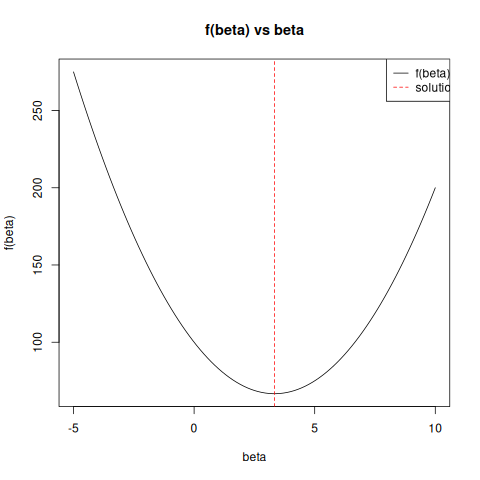
\includegraphics[scale=0.5]{ch6q6-0.png}
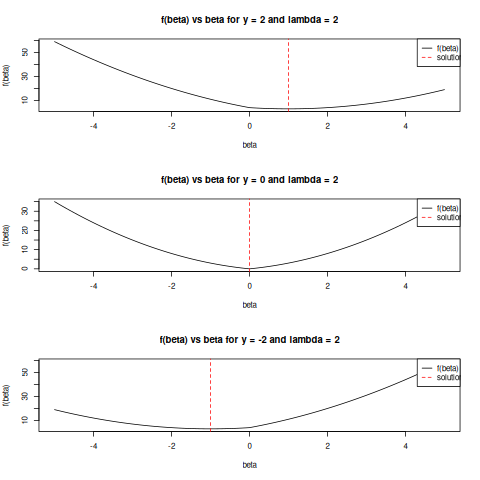
\includegraphics[scale=0.5]{ch6q6-1.png}

\newpage
\section{Chapter 6 - Applied 7}
\begin{enumerate}[label=(\alph*)]
\item 
\[ L(\vect \beta | \vect y, \vect X, \sigma) = \prod_{i=1}^{n} \frac{1}{\sqrt{2\pi\sigma^2}} \exp\left(-\frac{1}{2}(\vect y - \vect X \vect \beta)^T[\sigma^2 \vect I](\vect y - \vect X \vect\beta)\right) \]
where the first column of \(\vect X\) is 1
\item

Given \(p(\beta) = \frac{1}{2b}\exp(-\frac{|\beta|}{b})\)
Since independent, we have
\begin{align*}
p(\vect \beta) &= \prod_{i=1}^{p} \frac{1}{2b}\exp(-\frac{|\beta_i|}{b}) \\
&= \frac{1}{(2b)^p}\exp(-\frac{\norm{\vect \beta}_1}{b})
\end{align*}
Then we have
\[P(\vect \beta | \vect y, \vect X, b, \sigma) \propto 
(2\pi \sigma^2)^{-\frac{n}{2}}(2b)^{-p}\exp\left(-\frac{1}{2}(\vect y - \vect X \vect \beta)^T[\sigma^2 \vect I](\vect y - \vect X \vect\beta)\right) \exp(-\frac{\norm{\vect \beta}_1}{b})\]

To find the mode, we formulate the optimization problem
\begin{align*}
   \underset{\vect \beta}{\arg\max} P(\vect \beta | \vect y, \vect X, b, \sigma) 
   &= \underset{\vect \beta}{\arg\max} \log\left[ (2\pi \sigma^2)^{-\frac{n}{2}}(2b)^{-p}\exp\left(-\frac{1}{2}(\vect y - \vect X \vect \beta)^T[\sigma^2 \vect I](\vect y - \vect X \vect\beta)\right) \exp(-\frac{\norm{\vect \beta}_1}{b}) \right] \\
    &= \underset{\vect \beta}{\arg\min} \frac{(\vect y - \vect X \vect \beta)^T(\vect y - \vect X \vect\beta)}{2\sigma^2} + \frac{\norm{\vect \beta}_1}{b} \\
    &= \underset{\vect \beta}{\arg\min} (\vect y - \vect X \vect \beta)^T(\vect y - \vect X \vect\beta) + \frac{2\sigma^2}{b}\norm{\vect \beta}_1 \\
    &= \underset{\vect \beta}{\arg\min} \sum_{i=1}^n \left[ y_i - \sum_{i=0}^p \beta_j x_{ij}\right]^2 + \lambda\sum_{i=1}^p |\beta_j|
\end{align*}

This is the same as the Lasso problem with \(\lambda = \frac{2\sigma^2}{b}\) so the estimate will be the same as the Lasso estimate
\item
since \(\vect \beta\) is independently normally distributed, we have
\[P(\vect \beta | c) = \prod_{i=1}^{n} P(\beta_i \in \vect \beta | c) \propto \exp\left[-\frac{1}{2}\vect \beta^T [c\vect I]\vect \beta\right]\]

\begin{align*}
P(\vect \beta | \vect y,\vect X,c, \sigma^2) &\propto 
\exp [-\frac{1}{2\sigma^2} (\vect y - \vect X \vect \beta)^T(\vect y - \vect X \vect\beta) - \frac{1}{2c}\vect \beta^T\vect \beta ] \\
\end{align*}


Again we formulate the optimization problem

\begin{align*}
    \underset{\vect \beta}{\arg\max} P(\vect \beta | \vect y, \vect X, c, \sigma^2) 
    &= \underset{\vect \beta}{\arg\max} -\frac{1}{2\sigma^2} (\vect y - \vect X \vect \beta)^T(\vect y - \vect X \vect\beta) - \frac{1}{2c}\vect \beta^T \vect \beta  \\
    &= \underset{\vect \beta}{\arg\min} (\vect y - \vect X \vect \beta)^T(\vect y - \vect X \vect\beta) + \frac{\sigma^2}{c}\vect \beta^T \vect \beta  \\
    &= \underset{\vect \beta}{\arg\min} \sum_{i=1}^n \left[ y_i - \sum_{i=0}^p \beta_j x_{ij}\right]^2 + \lambda\sum_{i=1}^p \beta_j^2
\end{align*}

This is the same as the Ridge problem with \(\lambda = \frac{\sigma^2}{c}\) so the estimate will be the same as the Ridge estimate

\item
Since the ridge estimate is the solution to the optimization problem, the estimate is the mode of the posterior distribution

Now we to find the mode, we first show the posterior distribution follows normal distribution
\begin{align*}
P(\vect \beta | \vect y,\vect X,c, \sigma^2) &\propto 
\exp[-\frac{1}{2\sigma^2} (\vect y - \vect X \vect \beta)^T(\vect y - \vect X \vect\beta) - \frac{1}{2c}\vect \beta^T\vect \beta ]  \\
&= \exp[-\frac{1}{2\sigma^2}(\vect y^T\vect y - 2\vect y^T \vect X \vect \beta + \vect \beta^T \vect X^T \vect X \vect \beta) - \frac{1}{2c}\vect \beta^T\vect \beta ]\\
&= \exp[-\frac{1}{2\sigma^2}(\vect y^T\vect y) + \frac{1}{2}\vect \beta^T(\frac{1}{\sigma^2}\vect X^T \vect X + \frac{1}{c}\vect I)\vect \beta - 2\vect y^T \vect X \vect \beta] \\
&= \exp[-\frac{1}{2}(\vect \beta - \vect d)^T \vect \Omega^{-1}(\vect \beta - \vect d)] \\
\end{align*}

where \(\vect d = (\vect X^T \vect X + \sigma^2/c \vect I)\vect X^T \vect y\), \(\vect \Omega = \vect X^T \vect X + \frac{\sigma^2}{c}\vect I\)

This kernel shows that the posterior follows the normal distribution with mean \(\vect d\) and covariance \(\vect \Omega^{-1}\)

And mode and mean are the same for normal distribution, so the ridge estimate is also the mode of the posterior distribution

\end{enumerate}
\end{document}